\documentclass[12pt, a4paper]{article}
\usepackage{graphicx}
%
%Ours
\usepackage[USenglish]{babel}
\usepackage{todonotes}
\usepackage{etoolbox}
\usepackage{amsmath}
\usepackage{subfig}
\usepackage{tikz}
\usepackage{footnote}
\usepackage{amsmath}
\usepackage{float}
\usepackage{hhline}
\usepackage{cite}
\usepackage[inline]{enumitem}
\usepackage[all]{foreign}
\usepackage{nicefrac}
\usepackage[section]{placeins}
%\usepackage{showframe}
\usepackage{adjustbox}

%%% Style
% Font and layout
\newcommand*{\defemph}[1]{\ensuremath{\mathsf{#1}}}
\renewcommand*{\S}{Section}
\newcommand*{\sota}{state-of-the-art}
% Heavily used symbol style
\newcommand*{\agentstyle}[1]{{\ensuremath{\uppercase{\defemph{#1}}}}}
\newcommand*{\agentstyleMin}[1]{{\ensuremath{\lowercase{\defemph{#1}}}}}%}
\newcommand{\agent}[1]{%
  \ifstrequal{#1}{i}%
             {\ensuremath{\lowercase{\defemph{#1}}}}%
             {\ifstrequal{#1}{A}{\agentstyle{#1}}{%
\ifstrequal{#1}{a}{\agentstyle{#1}}{%
\ifstrequal{#1}{B}{\agentstyle{#1}}{%
\ifstrequal{#1}{b}{\agentstyle{#1}}{%
\ifstrequal{#1}{C}{\agentstyle{#1}}{%
\ifstrequal{#1}{c}{\agentstyle{#1}}{%
\ifstrequal{#1}{ag}{\agentstyleMin{#1}}{%
\ifstrequal{#1}{AG}{\agentstyleMin{#1}}{%
\ifstrequal{#1}{ag_1}{\agentstyleMin{#1}}{%
\ifstrequal{#1}{ag_2}{\agentstyleMin{#1}}{%
\ifstrequal{#1}{ag_i}{\agentstyleMin{#1}}{??
}}}}}}}}}}}}%
}
\newcommand*{\possarg}[2]{\ensuremath{\defemph{#1}(#2)}}
\newcommand*{\poss}[1]{\ensuremath{\defemph{#1}}}



%%% Operators, Actions and Syntax
% Epistemic logic operators
\newcommand*{\C}{\textbf{C}}
\newcommand*{\E}{\textbf{E}}
\newcommand*{\cAlpha}[1]{\ensuremath{\mathbf{C}_\alpha{#1}}}
\newcommand*{\eAlpha}[1]{\ensuremath{\mathbf{E}_\alpha{#1}}}
\newcommand*{\eAlphaIter}[2]{\ensuremath{\mathbf{E}^{#1}_\alpha{#2}}}
%\newcommand*{\initiallyC}[1]{\ensuremath{\texttt{initially\}(#1)}}
\newcommand*{\bB}[2]{\mathbf{B}_{\agent{#1}}{#2}}
\renewcommand*{\b}[1]{\ensuremath{\mathbf{B_{\agent{#1}}}}}
% Kripke operators
\newcommand*{\brel}[1]{\ensuremath{\calB_{\defemph{#1}}}}
\newcommand*{\rrel}[1]{\ensuremath{\calR_{\defemph{#1}}}}
% Actions and fluent
\newcommand*{\distract}[2]{%
\ifstrequal{#2}{}%
{\ensuremath{\mathtt{distract}(\agent{#1})}}%
{\ensuremath{\mathtt{distract}(\agent{#1})\langle\agent{#2}\rangle}}%
}
\newcommand*{\open}[1]{%
\ifstrequal{#1}{}%
{\ensuremath{\mathtt{open}}}%
{\ensuremath{\mathtt{open}\tuple{\agent{#1}}}}%
}
\newcommand*{\shout}[1]{%
\ifstrequal{#1}{}%
{\ensuremath{\mathtt{shout\_tails}}}%
{\ensuremath{\mathtt{shout\_tails}\tuple{\agent{#1}}}}%
}
\newcommand*{\signal}[2]{%
\ifstrequal{#2}{}%
{\ensuremath{\mathtt{signal}(\agent{#1})}}%
{\ensuremath{\mathtt{signal}(\agent{#1})\langle\agent{#2}\rangle}}%
}
\newcommand*{\peek}[1]{%
\ifstrequal{#1}{}%
{\ensuremath{\mathtt{peek}}}%
{\ensuremath{\mathtt{peek}\tuple{\agent{#1}}}}%
}
\newcommand*{\tell}[2]{%
\ifstrequal{#2}{}%
{\ensuremath{\mathtt{tell}(\agent{#1})}}%
{\ensuremath{\mathtt{tell}(\agent{#1})\langle\agent{#2}\rangle}}%
}
\newcommand*{\flip}[1]{%
\ifstrequal{#1}{}%
{\ensuremath{\mathtt{flip}}}%
{\ensuremath{\mathtt{flip}\tuple{\agent{#1}}}}%
}
\newcommand*{\haskey}[1]{\ensuremath{\mathtt{key}(\agent{#1})}}
\newcommand*{\opened}{\ensuremath{\mathtt{opened}}}
\newcommand*{\head}{\ensuremath{\mathtt{heads}}}
\newcommand*{\looking}[1]{\ensuremath{\mathtt{look}(\agent{#1})}}
\newcommand*{\res}[1]{\ensuremath{\defemph{caused}(\defemph{#1})}}
\newcommand*{\sensed}[2]{\ensuremath{\defemph{sensed}(\defemph{#1})[\defemph{#2}]}}
% Syntax
\newcommand*{\exec}[2]{\ensuremath{\mathbf{executable\ }\defemph{#1} \mathbf{\ if\ } #2 }}
\newcommand*{\causes}[2]{\ensuremath{\defemph{#1} \mathbf{\ causes\ } \defemph{#2} }}
\newcommand*{\determine}[2]{\ensuremath{\defemph{#1} \mathbf{\ determines\ } \defemph{#2} }}
\newcommand*{\announce}[2]{\ensuremath{\defemph{#1} \mathbf{\ announces\ } \defemph{#2} }}
\newcommand*{\initially}[1]{\ensuremath{\mathbf{intially}\ #1}}



%%% Special words
% Action languages
\newcommand*{\ourL}{\ensuremath{m\mathcal{A}^\rho}}
\newcommand*{\mAL}{\ensuremath{m\mathcal{A}^*}}
\newcommand*{\mAP}{\ensuremath{m\mathcal{A}+}}
% Multi agent epistemic
\newcommand*{\mAGep}{multi-agent epistemic}
\newcommand*{\MAGep}{Multi-agent epistemic}
\newcommand*{\ck}{common knowledge}
\newcommand*{\mep}{MEP}
% Non-well-founded set
\newcommand*{\Wf}{Well-founded}
\newcommand*{\wf}{well-founded}
\newcommand*{\Nwf}{Non-\wf}
\newcommand*{\nwf}{non-\wf}
%Possibilities & Co.
\newcommand*{\sPoss}{\ensuremath{\Phi_{\mathbf{Poss}}}}
\newcommand*{\Pos}{Possibility}
\newcommand*{\pos}{possibility}
\newcommand*{\PosS}{Possibilities}
\newcommand*{\posS}{possibilities}



%%%Special Symbols
% Languages
\newcommand*{\lAG}{\ensuremath{\mathcal{L}_{\sAG}}}
\newcommand*{\lag}{\lAG}
\newcommand*{\lagC}{\ensuremath{\lAG^{\C}}}
% Kripke structures
\newcommand*{\state}[2]{\ensuremath{(M_{\defemph{#1}},\defemph{#2})}}
\newcommand*{\posfunc}[3]{\ensuremath{\Phi_{D_{#1}}(#2,\defemph{#3})}}
\newcommand*{\trfunc}{\ensuremath{\Phi_D}}
\newcommand*{\posfull}{\ensuremath{F_{D}}}
\newcommand*{\pospartial}{\ensuremath{P_{D}}}
\newcommand*{\posoblivious}{\ensuremath{O_{D}}}
\newcommand*{\interp}[2]{\ensuremath{M_{#1}[\pi](\defemph #2)}}
% Special Sets
\newcommand*{\sAG}{\ensuremath{\mathcal{AG}}}
\newcommand*{\sAC}{\ensuremath{\mathcal{A}}}
\newcommand*{\sF}{\ensuremath{\mathcal{F}}}
\newcommand*{\sP}{\sF}
\newcommand*{\ai}{\calA\calI}
% Graph
\newcommand*{\graphG}{\ensuremath{\mathcal{G}}}
\newcommand*{\graphVE}[2]{\graphG=\textup{(}$#1, #2$\textup{)}}
% Generic
\newcommand*{\func}[3]{#1: #2 \mapsto #3}
\renewcommand*{\implies}{\ensuremath{\Rightarrow}}



%%% Shortcuts
\newcommand*{\bra}[1]{\ensuremath{\{#1\}}}
\newcommand*{\tuple}[1]{\ensuremath{\langle #1 \rangle}}



%%% Calligraphics macros by E. Zaffanella
\newcommand*{\calA}{\ensuremath{\mathcal{A}}}
\newcommand*{\calB}{\ensuremath{\mathcal{B}}}
\newcommand*{\calC}{\ensuremath{\mathcal{C}}}
\newcommand*{\calD}{\ensuremath{\mathcal{D}}}
\newcommand*{\calE}{\ensuremath{\mathcal{E}}}
\newcommand*{\calF}{\ensuremath{\mathcal{F}}}
\newcommand*{\calG}{\ensuremath{\mathcal{G}}}
\newcommand*{\calH}{\ensuremath{\mathcal{H}}}
\newcommand*{\calI}{\ensuremath{\mathcal{I}}}
\newcommand*{\calJ}{\ensuremath{\mathcal{J}}}
\newcommand*{\calK}{\ensuremath{\mathcal{K}}}
\newcommand*{\calL}{\ensuremath{\mathcal{L}}}
\newcommand*{\calM}{\ensuremath{\mathcal{M}}}
\newcommand*{\calN}{\ensuremath{\mathcal{N}}}
\newcommand*{\calO}{\ensuremath{\mathcal{O}}}
\newcommand*{\calP}{\ensuremath{\mathcal{P}}}
\newcommand*{\calQ}{\ensuremath{\mathcal{Q}}}
\newcommand*{\calR}{\ensuremath{\mathcal{R}}}
\newcommand*{\calS}{\ensuremath{\mathcal{S}}}
\newcommand*{\calT}{\ensuremath{\mathcal{T}}}
\newcommand*{\calU}{\ensuremath{\mathcal{U}}}
\newcommand*{\calV}{\ensuremath{\mathcal{V}}}
\newcommand*{\calW}{\ensuremath{\mathcal{W}}}
\newcommand*{\calX}{\ensuremath{\mathcal{X}}}
\newcommand*{\calY}{\ensuremath{\mathcal{Y}}}
\newcommand*{\calZ}{\ensuremath{\mathcal{Z}}}



%% Checkmark
\def\checkmark{\tikz\fill[scale=0.4](0,.35) -- (.25,0) -- (1,.7) -- (.25,.15) -- cycle;}

%%For SLIDES only
\newcommand*{\emphColorSlide}[1]{\textcolor{ForestGreen}{#1}}
\newcommand*{\emphSlide}[1]{\emphColorSlide{\emph{#1}}}
\newcommand*{\ttSlide}[1]{\textcolor{NavyBlue}{\texttt{#1}}}

\newcommand*{\colorAgentSlide}[1]{\textcolor{Black}{#1}}
\newcommand*{\agentSlide}[1]{%
\ifstrequal{#1}{Charlie}{\colorAgentSlide{\texttt{#1}}}%
{\ifstrequal{#1}{Lucy}{\colorAgentSlide{\texttt{#1}}}%
{\ifstrequal{#1}{Snoopy}{\colorAgentSlide{\texttt{#1}}}%
{\ifstrequal{#1}{ag}{\colorAgentSlide{\texttt{#1}}}%
{\ifstrequal{#1}{ag_i}{\ensuremath{\colorAgentSlide{\mathtt{#1}}}}%
{\ifstrequal{#1}{ag_1}{\ensuremath{\colorAgentSlide{\mathtt{#1}}}}%
{\ifstrequal{#1}{ag_2}{\ensuremath{\colorAgentSlide{\mathtt{#1}}}}%
{\ifstrequal{#1}{AG}{\colorAgentSlide{\texttt{\lowercase{#1}}}}%
{\ifstrequal{#1}{A}{\colorAgentSlide{\texttt{#1}}}%
{\ifstrequal{#1}{B}{\colorAgentSlide{\texttt{#1}}}%
{\ifstrequal{#1}{C}{\colorAgentSlide{\texttt{#1}}}%
{\ifstrequal{#1}{a}{\colorAgentSlide{\uppercase{\texttt{#1}}}}%
{\ifstrequal{#1}{b}{\colorAgentSlide{\uppercase{\texttt{#1}}}}%
{\ifstrequal{#1}{c}{\colorAgentSlide{\uppercase{\texttt{#1}}}}%
{\ifstrequal{#1}{agent}{\colorAgentSlide{\texttt{#1}}}%
{\ifstrequal{#1}{agents}{\colorAgentSlide{\texttt{#1}}}{??%
}}}}}}}}}}}}}}}}%
}
\newcommand*{\resSlide}[2]{\defemph{caused(#1)}[\ttSlide{#2}]}
\newcommand*{\sensedSlide}[2]{\defemph{sensed(#1)}[\ttSlide{#2}]}
\newcommand*{\brelSlide}[1]{\ensuremath{\calR_{\defemph{#1}}}}
\newcommand*{\bBSlide}[2]{\mathbf{B}_{\texttt{#1}}{#2}}
\newcommand{\showCILC}[2]{%
	\ifstrequal{#1}{true}{#2}{}}


%\full (Azione, pointed kripke structure(2 argomenti), insieme  )
%\newcommand*{\Interp}[2]{\ensuremath{M_{#1}[\pi](#2)}}
%\newcommand*{\nwfeq}[3]{\ensuremath{#1(#2)=#3}}


%
%
%
\begin{document}

\begin{figure}[H]
	\centering
	

\tikzset{every picture/.style={line width=0.75pt}} %set default line width to 0.75pt        

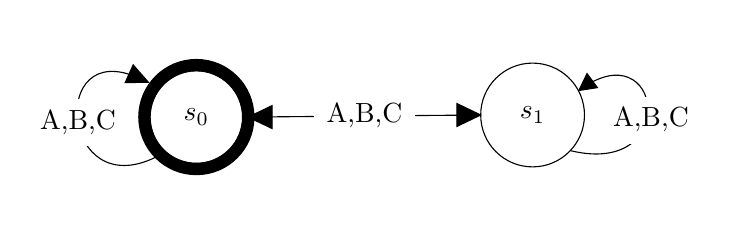
\begin{tikzpicture}[x=0.75pt,y=0.75pt,yscale=-1,xscale=1]
%uncomment if require: \path (0,300); %set diagram left start at 0, and has height of 300

%Shape: Circle [id:dp03041330611239501] 
\draw   (100,136) .. controls (100,122.19) and (111.19,111) .. (125,111) .. controls (138.81,111) and (150,122.19) .. (150,136) .. controls (150,149.81) and (138.81,161) .. (125,161) .. controls (111.19,161) and (100,149.81) .. (100,136) -- cycle ;
%Shape: Circle [id:dp06778329694496121] 
\draw   (262,135) .. controls (262,121.19) and (273.19,110) .. (287,110) .. controls (300.81,110) and (312,121.19) .. (312,135) .. controls (312,148.81) and (300.81,160) .. (287,160) .. controls (273.19,160) and (262,148.81) .. (262,135) -- cycle ;
%Straight Lines [id:da33786910107719414] 
\draw    (262,135) -- (150,136) ;


%Shape: Circle [id:dp28310457724521987] 
\draw   (102.6,136) .. controls (102.6,123.63) and (112.63,113.6) .. (125,113.6) .. controls (137.37,113.6) and (147.4,123.63) .. (147.4,136) .. controls (147.4,148.37) and (137.37,158.4) .. (125,158.4) .. controls (112.63,158.4) and (102.6,148.37) .. (102.6,136) -- cycle ;
%Shape: Circle [id:dp9488628075819832] 
\draw  [line width=4.5]  (100,136) .. controls (100,122.19) and (111.19,111) .. (125,111) .. controls (138.81,111) and (150,122.19) .. (150,136) .. controls (150,149.81) and (138.81,161) .. (125,161) .. controls (111.19,161) and (100,149.81) .. (100,136) -- cycle ;
%Curve Lines [id:da15096966683993052] 
\draw    (105.72,155.18) .. controls (59.72,178.18) and (53.3,97.2) .. (97.3,117.2) ;


%Shape: Triangle [id:dp024620734385268905] 
\draw  [fill={rgb, 255:red, 0; green, 0; blue, 0 }  ,fill opacity=1 ] (101.95,119.29) -- (90.74,119.35) -- (94.56,110.87) -- cycle ;
%Curve Lines [id:da3650058854241438] 
\draw    (309.3,123.2) .. controls (349.3,93.2) and (359.3,165.2) .. (305.3,152.2) ;


%Shape: Triangle [id:dp6528725824186807] 
\draw  [fill={rgb, 255:red, 0; green, 0; blue, 0 }  ,fill opacity=1 ] (309.3,123.2) -- (313.22,115.05) -- (318.23,121.81) -- cycle ;
%Shape: Triangle [id:dp5954374173670742] 
\draw  [fill={rgb, 255:red, 0; green, 0; blue, 0 }  ,fill opacity=1 ] (262,135) -- (250.5,140.53) -- (250.5,129.47) -- cycle ;
%Shape: Triangle [id:dp7130809704304564] 
\draw  [fill={rgb, 255:red, 0; green, 0; blue, 0 }  ,fill opacity=1 ] (150,136) -- (161.5,130.47) -- (161.5,141.53) -- cycle ;

% Text Node
\draw (125,136) node  [align=left] {$s_0$};
% Text Node
\draw (287,135) node  [align=left] {$s_1$};
% Text Node
\draw  [color={rgb, 255:red, 255; green, 255; blue, 255 }  ,draw opacity=1 ][fill={rgb, 255:red, 255; green, 255; blue, 255 }  ,fill opacity=1 ]  (182,124.5) -- (230,124.5) -- (230,146.5) -- (182,146.5) -- cycle  ;
\draw (206,135.5) node  [align=left] {A,B,C};
% Text Node
\draw  [color={rgb, 255:red, 255; green, 255; blue, 255 }  ,draw opacity=1 ][fill={rgb, 255:red, 255; green, 255; blue, 255 }  ,fill opacity=1 ]  (44,127.5) -- (92,127.5) -- (92,149.5) -- (44,149.5) -- cycle  ;
\draw (68,138.5) node  [align=left] {A,B,C};
% Text Node
\draw  [color={rgb, 255:red, 255; green, 255; blue, 255 }  ,draw opacity=1 ][fill={rgb, 255:red, 255; green, 255; blue, 255 }  ,fill opacity=1 ]  (320,126.5) -- (368,126.5) -- (368,148.5) -- (320,148.5) -- cycle  ;
\draw (344,137.5) node  [align=left] {A,B,C};


\end{tikzpicture}

	\caption{Initial State.}
\end{figure}%
\begin{align*}
s_0 &= \bra{\looking b,\looking c, \opened}\\
s_1 &= \bra{\looking{b},\looking{c},\opened,\head}
\end{align*}

\begin{figure}[H]
	\centering
	

\tikzset{every picture/.style={line width=0.75pt}} %set default line width to 0.75pt        

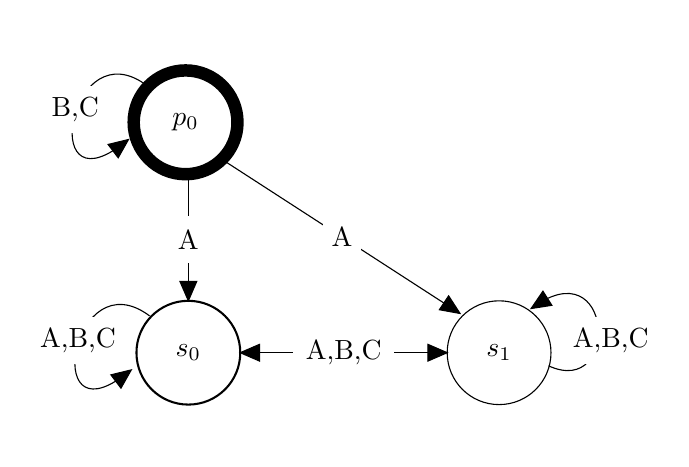
\begin{tikzpicture}[x=0.75pt,y=0.75pt,yscale=-1,xscale=1]
%uncomment if require: \path (0,300); %set diagram left start at 0, and has height of 300

%Shape: Circle [id:dp8938158972072578] 
\draw  [line width=0.75]  (105.29,143) .. controls (105.29,129.19) and (116.48,118) .. (130.29,118) .. controls (144.09,118) and (155.29,129.19) .. (155.29,143) .. controls (155.29,156.81) and (144.09,168) .. (130.29,168) .. controls (116.48,168) and (105.29,156.81) .. (105.29,143) -- cycle ;
%Shape: Circle [id:dp19780391712041556] 
\draw   (255,143) .. controls (255,129.19) and (266.19,118) .. (280,118) .. controls (293.81,118) and (305,129.19) .. (305,143) .. controls (305,156.81) and (293.81,168) .. (280,168) .. controls (266.19,168) and (255,156.81) .. (255,143) -- cycle ;
%Straight Lines [id:da018251469869151382] 
\draw    (155.29,143) -- (255,143) ;


%Shape: Triangle [id:dp4725710951486233] 
\draw  [fill={rgb, 255:red, 0; green, 0; blue, 0 }  ,fill opacity=1 ] (102.8,151.28) -- (97.82,160.08) -- (92.97,153.67) -- cycle ;
%Shape: Triangle [id:dp08394946096129607] 
\draw  [fill={rgb, 255:red, 0; green, 0; blue, 0 }  ,fill opacity=1 ] (255,143) -- (245.72,147.02) -- (245.72,138.98) -- cycle ;
%Shape: Triangle [id:dp12888926826248426] 
\draw  [fill={rgb, 255:red, 0; green, 0; blue, 0 }  ,fill opacity=1 ] (155.29,143) -- (164.56,138.98) -- (164.56,147.02) -- cycle ;
%Shape: Triangle [id:dp7536519811814515] 
\draw  [fill={rgb, 255:red, 0; green, 0; blue, 0 }  ,fill opacity=1 ] (295.43,121.72) -- (301.13,113.37) -- (305.42,120.17) -- cycle ;
%Curve Lines [id:da0862450190271058] 
\draw    (111.62,125.27) .. controls (74.82,97.67) and (59.1,184.08) .. (99.1,154.08) ;


%Curve Lines [id:da8507870813478686] 
\draw    (295.43,121.72) .. controls (335.43,91.72) and (338.63,165.32) .. (303.83,149.32) ;


%Shape: Circle [id:dp06782137726568571] 
\draw  [line width=4.5]  (103.95,32) .. controls (103.95,18.19) and (115.15,7) .. (128.95,7) .. controls (142.76,7) and (153.95,18.19) .. (153.95,32) .. controls (153.95,45.81) and (142.76,57) .. (128.95,57) .. controls (115.15,57) and (103.95,45.81) .. (103.95,32) -- cycle ;
%Shape: Triangle [id:dp8413979641210945] 
\draw  [fill={rgb, 255:red, 0; green, 0; blue, 0 }  ,fill opacity=1 ] (101.46,40.28) -- (96.49,49.08) -- (91.64,42.67) -- cycle ;
%Shape: Triangle [id:dp7368099608094223] 
\draw  [fill={rgb, 255:red, 0; green, 0; blue, 0 }  ,fill opacity=1 ] (261.18,124.1) -- (251.23,122.29) -- (255.69,115.61) -- cycle ;
%Curve Lines [id:da6315070066186073] 
\draw    (110.29,14.27) .. controls (73.49,-13.33) and (57.76,73.08) .. (97.76,43.08) ;


%Straight Lines [id:da7382395640533164] 
\draw    (130.29,59) -- (130.29,118) ;


%Straight Lines [id:da3690444677581517] 
\draw    (147.37,50.44) -- (261.18,124.1) ;


%Shape: Triangle [id:dp417855807516911] 
\draw  [fill={rgb, 255:red, 0; green, 0; blue, 0 }  ,fill opacity=1 ] (130.29,118) -- (126.27,108.72) -- (134.3,108.72) -- cycle ;

% Text Node
\draw (130.29,143) node  [align=left] {$s_0$};
% Text Node
\draw (280,143) node  [align=left] {$s_1$};
% Text Node
\draw  [color={rgb, 255:red, 255; green, 255; blue, 255 }  ,draw opacity=1 ][fill={rgb, 255:red, 255; green, 255; blue, 255 }  ,fill opacity=1 ]  (181.14,132) -- (229.14,132) -- (229.14,154) -- (181.14,154) -- cycle  ;
\draw (205.14,143) node  [align=left] {A,B,C};
% Text Node
\draw  [color={rgb, 255:red, 255; green, 255; blue, 255 }  ,draw opacity=1 ][fill={rgb, 255:red, 255; green, 255; blue, 255 }  ,fill opacity=1 ]  (53.14,126) -- (101.14,126) -- (101.14,148) -- (53.14,148) -- cycle  ;
\draw (77.14,137) node  [align=left] {A,B,C};
% Text Node
\draw  [color={rgb, 255:red, 255; green, 255; blue, 255 }  ,draw opacity=1 ][fill={rgb, 255:red, 255; green, 255; blue, 255 }  ,fill opacity=1 ]  (309.81,126) -- (357.81,126) -- (357.81,148) -- (309.81,148) -- cycle  ;
\draw (333.81,137) node  [align=left] {A,B,C};
% Text Node
\draw (128.95,32) node  [align=left] {$p_0$};
% Text Node
\draw  [color={rgb, 255:red, 255; green, 255; blue, 255 }  ,draw opacity=1 ][fill={rgb, 255:red, 255; green, 255; blue, 255 }  ,fill opacity=1 ]  (59.31,15) -- (92.31,15) -- (92.31,37) -- (59.31,37) -- cycle  ;
\draw (75.81,26) node  [align=left] {B,C};
% Text Node
\draw  [color={rgb, 255:red, 255; green, 255; blue, 255 }  ,draw opacity=1 ][fill={rgb, 255:red, 255; green, 255; blue, 255 }  ,fill opacity=1 ]  (121.29,77.5) -- (139.29,77.5) -- (139.29,99.5) -- (121.29,99.5) -- cycle  ;
\draw (130.29,88.5) node  [align=left] {A};
% Text Node
\draw  [color={rgb, 255:red, 255; green, 255; blue, 255 }  ,draw opacity=1 ][fill={rgb, 255:red, 255; green, 255; blue, 255 }  ,fill opacity=1 ]  (195.27,76.27) -- (213.27,76.27) -- (213.27,98.27) -- (195.27,98.27) -- cycle  ;
\draw (204.27,87.27) node  [align=left] {A};


\end{tikzpicture}

	\caption{State after \peek{B} where $p_0 = \bra{\looking b,\looking c, \opened}$.}
\end{figure}%


\begin{figure}[H]
	\centering
	\input{distract}
	\caption{State after \distract{B}{C} where $q_0 = \bra{\looking c, \opened}$.}
\end{figure}%


\begin{figure}[H]
	\centering
	

\tikzset{every picture/.style={line width=0.75pt}} %set default line width to 0.75pt        

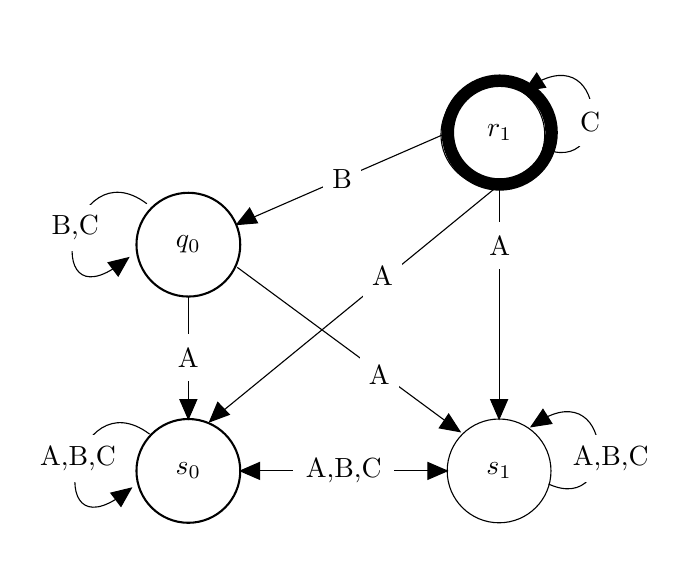
\begin{tikzpicture}[x=0.75pt,y=0.75pt,yscale=-1,xscale=1]
%uncomment if require: \path (0,300); %set diagram left start at 0, and has height of 300

%Shape: Circle [id:dp8938158972072578] 
\draw  [line width=0.75]  (135.29,223) .. controls (135.29,209.19) and (146.48,198) .. (160.29,198) .. controls (174.09,198) and (185.29,209.19) .. (185.29,223) .. controls (185.29,236.81) and (174.09,248) .. (160.29,248) .. controls (146.48,248) and (135.29,236.81) .. (135.29,223) -- cycle ;
%Shape: Circle [id:dp19780391712041556] 
\draw   (285,223) .. controls (285,209.19) and (296.19,198) .. (310,198) .. controls (323.81,198) and (335,209.19) .. (335,223) .. controls (335,236.81) and (323.81,248) .. (310,248) .. controls (296.19,248) and (285,236.81) .. (285,223) -- cycle ;
%Straight Lines [id:da018251469869151382] 
\draw    (185.29,223) -- (285,223) ;


%Shape: Triangle [id:dp4725710951486233] 
\draw  [fill={rgb, 255:red, 0; green, 0; blue, 0 }  ,fill opacity=1 ] (132.8,231.28) -- (127.82,240.08) -- (122.97,233.67) -- cycle ;
%Shape: Triangle [id:dp08394946096129607] 
\draw  [fill={rgb, 255:red, 0; green, 0; blue, 0 }  ,fill opacity=1 ] (285,223) -- (275.72,227.02) -- (275.72,218.98) -- cycle ;
%Shape: Triangle [id:dp12888926826248426] 
\draw  [fill={rgb, 255:red, 0; green, 0; blue, 0 }  ,fill opacity=1 ] (185.29,223) -- (194.56,218.98) -- (194.56,227.02) -- cycle ;
%Shape: Triangle [id:dp7536519811814515] 
\draw  [fill={rgb, 255:red, 0; green, 0; blue, 0 }  ,fill opacity=1 ] (325.43,201.72) -- (331.13,193.37) -- (335.42,200.17) -- cycle ;
%Curve Lines [id:da0862450190271058] 
\draw    (141.62,205.27) .. controls (104.82,177.67) and (89.1,264.08) .. (129.1,234.08) ;


%Curve Lines [id:da8507870813478686] 
\draw    (325.43,201.72) .. controls (365.43,171.72) and (368.63,245.32) .. (333.83,229.32) ;


%Shape: Circle [id:dp06782137726568571] 
\draw  [line width=0.75]  (135.29,114) .. controls (135.29,100.19) and (146.48,89) .. (160.29,89) .. controls (174.09,89) and (185.29,100.19) .. (185.29,114) .. controls (185.29,127.81) and (174.09,139) .. (160.29,139) .. controls (146.48,139) and (135.29,127.81) .. (135.29,114) -- cycle ;
%Shape: Triangle [id:dp8413979641210945] 
\draw  [fill={rgb, 255:red, 0; green, 0; blue, 0 }  ,fill opacity=1 ] (131.46,120.28) -- (126.49,129.08) -- (121.64,122.67) -- cycle ;
%Shape: Triangle [id:dp7368099608094223] 
\draw  [fill={rgb, 255:red, 0; green, 0; blue, 0 }  ,fill opacity=1 ] (291.18,204.1) -- (281.23,202.29) -- (285.69,195.61) -- cycle ;
%Curve Lines [id:da6315070066186073] 
\draw    (140.29,94.27) .. controls (103.49,66.67) and (87.76,153.08) .. (127.76,123.08) ;


%Straight Lines [id:da7382395640533164] 
\draw    (160.29,139) -- (160.29,198) ;


%Straight Lines [id:da3690444677581517] 
\draw    (183.87,124.94) -- (291.18,204.1) ;


%Shape: Triangle [id:dp417855807516911] 
\draw  [fill={rgb, 255:red, 0; green, 0; blue, 0 }  ,fill opacity=1 ] (160.29,198) -- (156.27,188.72) -- (164.3,188.72) -- cycle ;
%Shape: Circle [id:dp5972014220045965] 
\draw  [line width=4.5]  (285.29,60) .. controls (285.29,46.19) and (296.48,35) .. (310.29,35) .. controls (324.09,35) and (335.29,46.19) .. (335.29,60) .. controls (335.29,73.81) and (324.09,85) .. (310.29,85) .. controls (296.48,85) and (285.29,73.81) .. (285.29,60) -- cycle ;
%Shape: Triangle [id:dp4971926593318259] 
\draw  [fill={rgb, 255:red, 0; green, 0; blue, 0 }  ,fill opacity=1 ] (170.53,199.33) -- (174.44,190.01) -- (180.01,195.81) -- cycle ;
%Straight Lines [id:da46185098746714237] 
\draw    (310.29,85) -- (310.29,193.36) ;


%Straight Lines [id:da9004694794581629] 
\draw    (310.29,85) -- (170.53,199.33) ;


%Shape: Triangle [id:dp3663238051701312] 
\draw  [fill={rgb, 255:red, 0; green, 0; blue, 0 }  ,fill opacity=1 ] (310,198) -- (305.98,188.72) -- (314.02,188.72) -- cycle ;
%Shape: Circle [id:dp9462184779936802] 
\draw   (282,61) .. controls (282,47.19) and (293.19,36) .. (307,36) .. controls (320.81,36) and (332,47.19) .. (332,61) .. controls (332,74.81) and (320.81,86) .. (307,86) .. controls (293.19,86) and (282,74.81) .. (282,61) -- cycle ;
%Shape: Triangle [id:dp5745677700051097] 
\draw  [fill={rgb, 255:red, 0; green, 0; blue, 0 }  ,fill opacity=1 ] (322.43,39.72) -- (328.13,31.37) -- (332.42,38.17) -- cycle ;
%Curve Lines [id:da6922101751426857] 
\draw    (322.43,39.72) .. controls (362.43,9.72) and (365.63,83.32) .. (330.83,67.32) ;


%Straight Lines [id:da08547301161768894] 
\draw    (285.29,60) -- (183.53,104.33) ;


%Shape: Triangle [id:dp20482466216590445] 
\draw  [fill={rgb, 255:red, 0; green, 0; blue, 0 }  ,fill opacity=1 ] (183.53,104.33) -- (189.81,96.41) -- (193.6,103.49) -- cycle ;

% Text Node
\draw (160.29,223) node  [align=left] {$s_0$};
% Text Node
\draw (310,223) node  [align=left] {$s_1$};
% Text Node
\draw  [color={rgb, 255:red, 255; green, 255; blue, 255 }  ,draw opacity=1 ][fill={rgb, 255:red, 255; green, 255; blue, 255 }  ,fill opacity=1 ]  (211.14,212) -- (259.14,212) -- (259.14,234) -- (211.14,234) -- cycle  ;
\draw (235.14,223) node  [align=left] {A,B,C};
% Text Node
\draw  [color={rgb, 255:red, 255; green, 255; blue, 255 }  ,draw opacity=1 ][fill={rgb, 255:red, 255; green, 255; blue, 255 }  ,fill opacity=1 ]  (83.14,206) -- (131.14,206) -- (131.14,228) -- (83.14,228) -- cycle  ;
\draw (107.14,217) node  [align=left] {A,B,C};
% Text Node
\draw  [color={rgb, 255:red, 255; green, 255; blue, 255 }  ,draw opacity=1 ][fill={rgb, 255:red, 255; green, 255; blue, 255 }  ,fill opacity=1 ]  (339.81,206) -- (387.81,206) -- (387.81,228) -- (339.81,228) -- cycle  ;
\draw (363.81,217) node  [align=left] {A,B,C};
% Text Node
\draw (160.29,114) node  [align=left] {$q_0$};
% Text Node
\draw  [color={rgb, 255:red, 255; green, 255; blue, 255 }  ,draw opacity=1 ][fill={rgb, 255:red, 255; green, 255; blue, 255 }  ,fill opacity=1 ]  (89.31,95) -- (122.31,95) -- (122.31,117) -- (89.31,117) -- cycle  ;
\draw (105.81,106) node  [align=left] {B,C};
% Text Node
\draw  [color={rgb, 255:red, 255; green, 255; blue, 255 }  ,draw opacity=1 ][fill={rgb, 255:red, 255; green, 255; blue, 255 }  ,fill opacity=1 ]  (151.29,157.5) -- (169.29,157.5) -- (169.29,179.5) -- (151.29,179.5) -- cycle  ;
\draw (160.29,168.5) node  [align=left] {A};
% Text Node
\draw  [color={rgb, 255:red, 255; green, 255; blue, 255 }  ,draw opacity=1 ][fill={rgb, 255:red, 255; green, 255; blue, 255 }  ,fill opacity=1 ]  (243.27,165.77) -- (261.27,165.77) -- (261.27,187.77) -- (243.27,187.77) -- cycle  ;
\draw (252.27,176.77) node  [align=left] {A};
% Text Node
\draw (310.29,60) node  [align=left] {$r_1$};
% Text Node
\draw  [color={rgb, 255:red, 255; green, 255; blue, 255 }  ,draw opacity=1 ][fill={rgb, 255:red, 255; green, 255; blue, 255 }  ,fill opacity=1 ]  (301.29,103.5) -- (319.29,103.5) -- (319.29,125.5) -- (301.29,125.5) -- cycle  ;
\draw (310.29,114.5) node  [align=left] {A};
% Text Node
\draw  [color={rgb, 255:red, 255; green, 255; blue, 255 }  ,draw opacity=1 ][fill={rgb, 255:red, 255; green, 255; blue, 255 }  ,fill opacity=1 ]  (244.77,118.27) -- (262.77,118.27) -- (262.77,140.27) -- (244.77,140.27) -- cycle  ;
\draw (253.77,129.27) node  [align=left] {A};
% Text Node
\draw  [color={rgb, 255:red, 255; green, 255; blue, 255 }  ,draw opacity=1 ][fill={rgb, 255:red, 255; green, 255; blue, 255 }  ,fill opacity=1 ]  (344.31,44) -- (363.31,44) -- (363.31,66) -- (344.31,66) -- cycle  ;
\draw (353.81,55) node  [align=left] {C};
% Text Node
\draw  [color={rgb, 255:red, 255; green, 255; blue, 255 }  ,draw opacity=1 ][fill={rgb, 255:red, 255; green, 255; blue, 255 }  ,fill opacity=1 ]  (225.41,71.17) -- (243.41,71.17) -- (243.41,93.17) -- (225.41,93.17) -- cycle  ;
\draw (234.41,82.17) node  [align=left] {B};


\end{tikzpicture}

	\caption{State after \flip{C} where $r_1 = \bra{\looking c, \opened, \head}$.}
\end{figure}%


\begin{figure}[H]
	\centering
	\input{tell}
	\caption{State after \tell{B}{c}.}
\end{figure}%

\end{document}
